% RESULTADOS-------------------------------------------------------------------

\chapter{RESULTADOS}
\label{chap:resultados}

Nesse capitulo será discutido brevemente os resultados globais obtidos com o desenvolvimento do protótipo e mostrado um teste comparativo entre dois \textit{codecs} de video testados com a biblioteca \textit{FFmpeg}.\par

\subsection{Resultados Globais}
\label{subsec:resglobais}

De modo geral, o protótipo se comportou conforme o esperado. A captura de movimento da cabeça do operador funciona de maneira satisfatória e os motores respondem sem atrasos perceptíveis (que representassem desconforto ao operador).\par

Por outro lado, o sistema de envio de imagens precisa ser optimizado. Talvez um dispositivo de captura com mais qualidade, como o módulo de câmera oficial do Raspverry Pi, que possui um drive especifico implementado em hardware, represente uma melhoria no sistema global de captura e enfio de imagens capturadas.\par

O consumo da banda de dados, durante o envio de coordenadas, foi minimizado pela aplicação de um filtro que compara a última coordenada válida com a que será enviada. Desse modo somente as modificações de posição são enviadas ao módulo de controle de câmeras.\par

Os eventos, gerados pela API do Android, ocorrem em um tempo especificado pelo desenvolvedor. Para identificar esse tempo, levou-se em consideração a responsividade necessária para os motores e o uso de banda de dados. Quando menor o intervalo de tempo entre os eventos, maior é a resolução do dado e maior o consumo de banda de dados. Para chegar-se a um valor adequado, testes práticos foram feitos variando-se o intervalo de eventos entre 10 e 500 milissegundos. Chegou-se a conclusão que valores entre 30 e 90 milissegundos são satisfatórios.\par

\subsection{Comparação Entre \textit{codecs}}
\label{subsec:compcodecs}

Dentre os testes realizados com alguns dos \textit{codecs} de vídeo compatíveis com o FFmpeg, os que mais chamaram atenção e que representaram um ganho considerável foram o \textbf{h264\_omx} e \textbf{h264}, implementados em hardware e software respectivamente.
Comparando-se a \autoref{fig:top_ffmpeg_h264} e a \autoref{fig:top_ffmpeg_h264_omx}, obtidas da interface do gerenciador de tarefas \textit{top}, fica claro que a implementação de \textit{codecs} via hardware traz um ganho, em tempo de processador e quantidade de memoria \textit{RAM} alocada, considerável. Existe um ganho de aproximadamente 28\% em tempo de processador e 35\% em uso de memoria \textit{RAM}. Uma parte do uso de recursos nas duas figuras está relacionada ao processo de \textit{streaming}, implementada via software. Como o \textit{streaming} é o mesmo para as duas comparações, não existe inconsistência na comparação.

\begin{figure}[H]
	\centering
	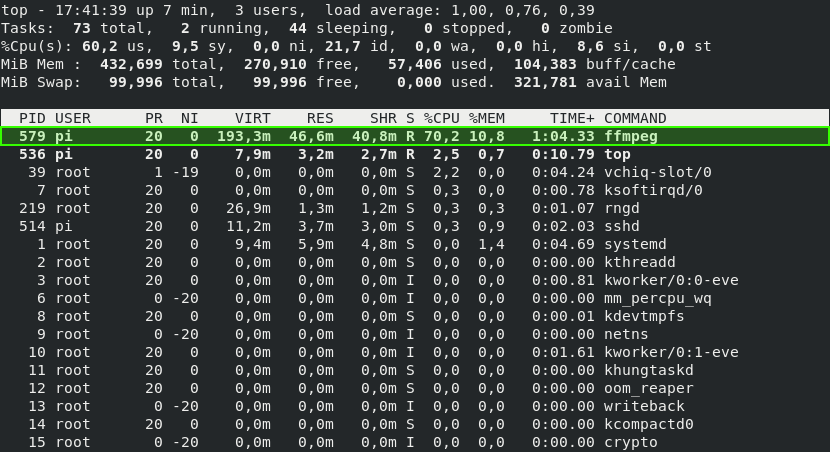
\includegraphics[width=1\textwidth]{figuras/top_ffmpeg_h264_omx.png}
	\caption{Consumo de recursos de hardware pelo FFmpeg usando o codec h264\_omx, implementado em hardware.}
	\label{fig:top_ffmpeg_h264_omx}
\end{figure}

\begin{figure}[H]
	\centering
	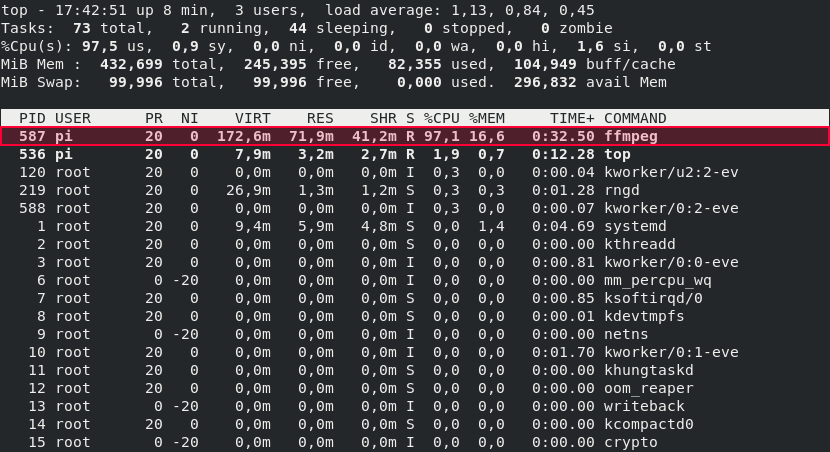
\includegraphics[width=1\textwidth]{figuras/top_ffmpeg_h264.png}
	\caption{Consumo de recursos de hardware pelo FFmpeg usando o codec h264, implementado em software.}
	\label{fig:top_ffmpeg_h264}
\end{figure}

\begin{figure}[H]
	\centering
	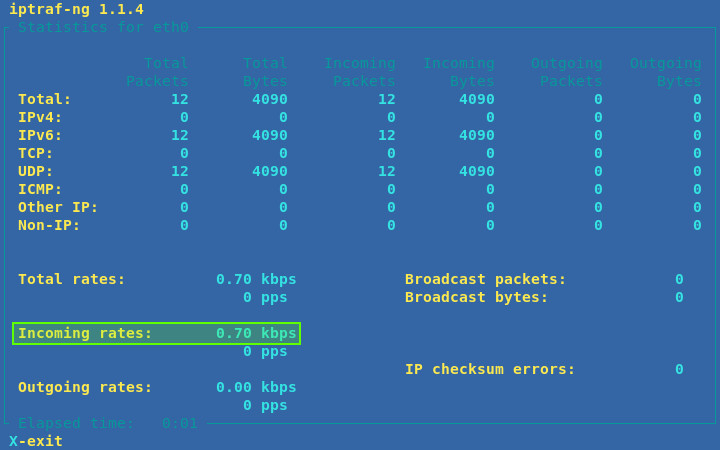
\includegraphics[width=1\textwidth]{figuras/consumo_banda.jpg}
	\caption{Consumo dos recursos de rede durante o recebimento de coordenadas.}
	\label{fig:consumo_banda}
\end{figure}

\begin{figure}[H]
	\centering
	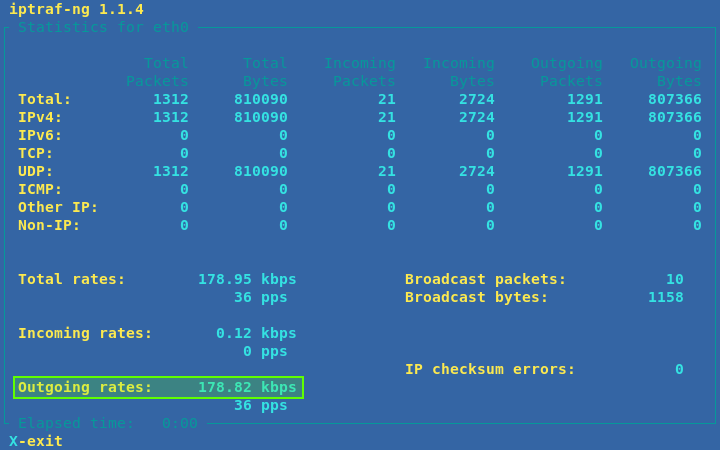
\includegraphics[width=1\textwidth]{figuras/consumo_banda_camera.png}
	\caption{Consumo dos recursos de rede durante o envio de imagem da câmera.}
	\label{fig:consumo_banda}
\end{figure}



\begin{comment}

\section{Análise modal numérica}
\label{sec:resultmodal}

Na análise modal, as frequências naturais obtidas para os dois casos mantiveram-se afastadas da faixa de operação da turbina. Considerando uma TSR entre 2 e 3,5 e uma faixa de velocidade comumente encontrada entre 1 e 2 $m/s$ tem-se uma faixa de frequências de operação variando entre 0,62 e 2,16 $Hz$ que se encontra distante das frequências naturais encontradas para os casos analisados conforme apresentado na \autoref{tab:resultfreqturbina}. Tal verificação vem confirmar a possibilidade de utilização da consideração de 1 GDL. 

\begin{table}[h]
	\centering
	\caption{Frequências naturais obtidas [Hz].}
	\label{tab:resultfreqturbina}	
	    \begin{tabular}{c c c}
        \hline Modo &  &  \\
         & Maciço & Tubo \\
        \hline        
		1 & 9,04 & 7,54 \\
		2 & 9,08 & 7,55 \\
		3 & 13,40 & 9,80 \\
		4 & 28,68 & 20,19\\
		5 & 28,74 & 20,21 \\
		6 & 30,32 & 24,56 \\
		\hline
    \end{tabular}

	\fonte{Autoria própria.}
\end{table}

As \autoref{fig:resultmodomacico} e \autoref{fig:resultmodotubos} apresentam algumas respostas esperadas para o primeiro e sexto modo de vibração. Nelas é possível verificar a importância da verificação das frequências de operação da turbina, que caso negligenciado pode levar a sérios danos. Também pode-se verificar que a utilização do tubo em comparação aos eixos maciços levaram a maiores deformações.    

\begin{figure}	
	\caption{Modos de vibração do sistema com eixo e braço maciços.}
	\label{fig:resultmodomacico}
	\begin{subfigure}{0.5\textwidth}
		\centering
		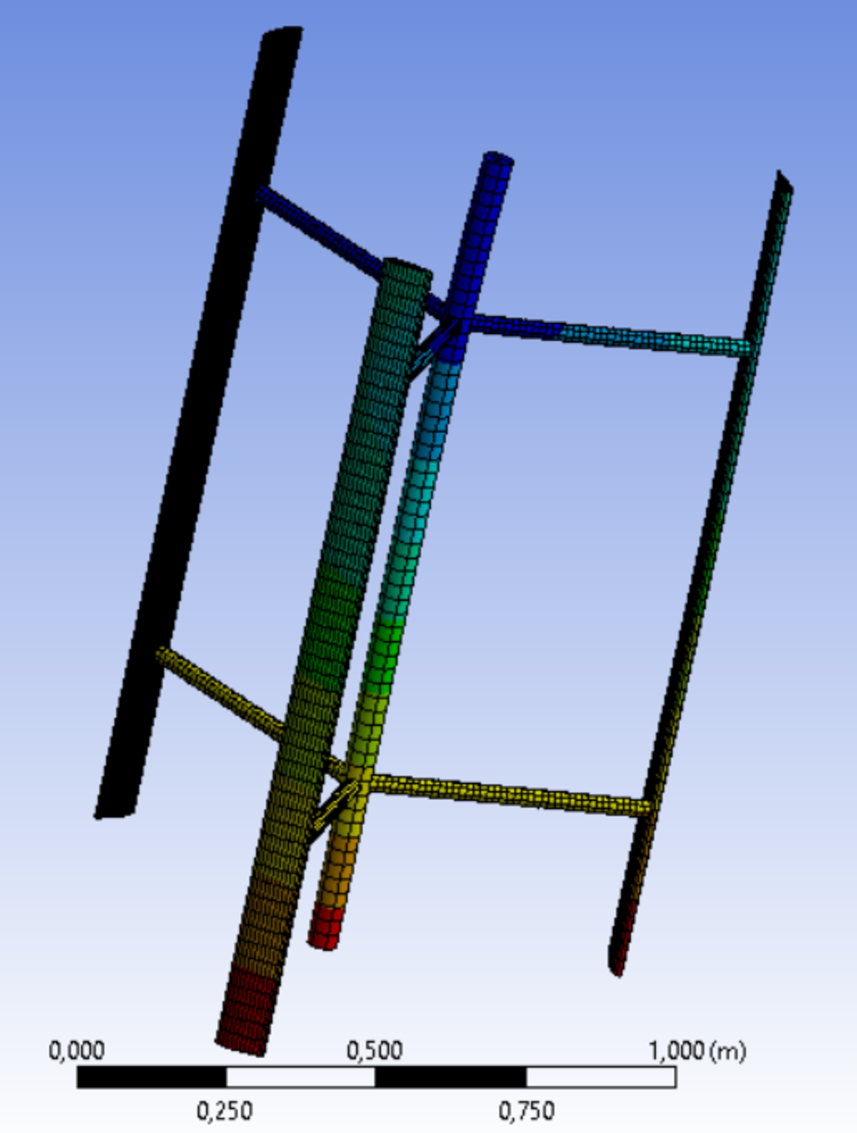
\includegraphics[width=1.0\textwidth]{figuras/resultmodalmacico1.pdf}
		\caption{Primeiro modo.}
		\label{subfig:resultmodomacicomodo1}
	\end{subfigure}
	\begin{subfigure}{0.5\textwidth}
		\centering
		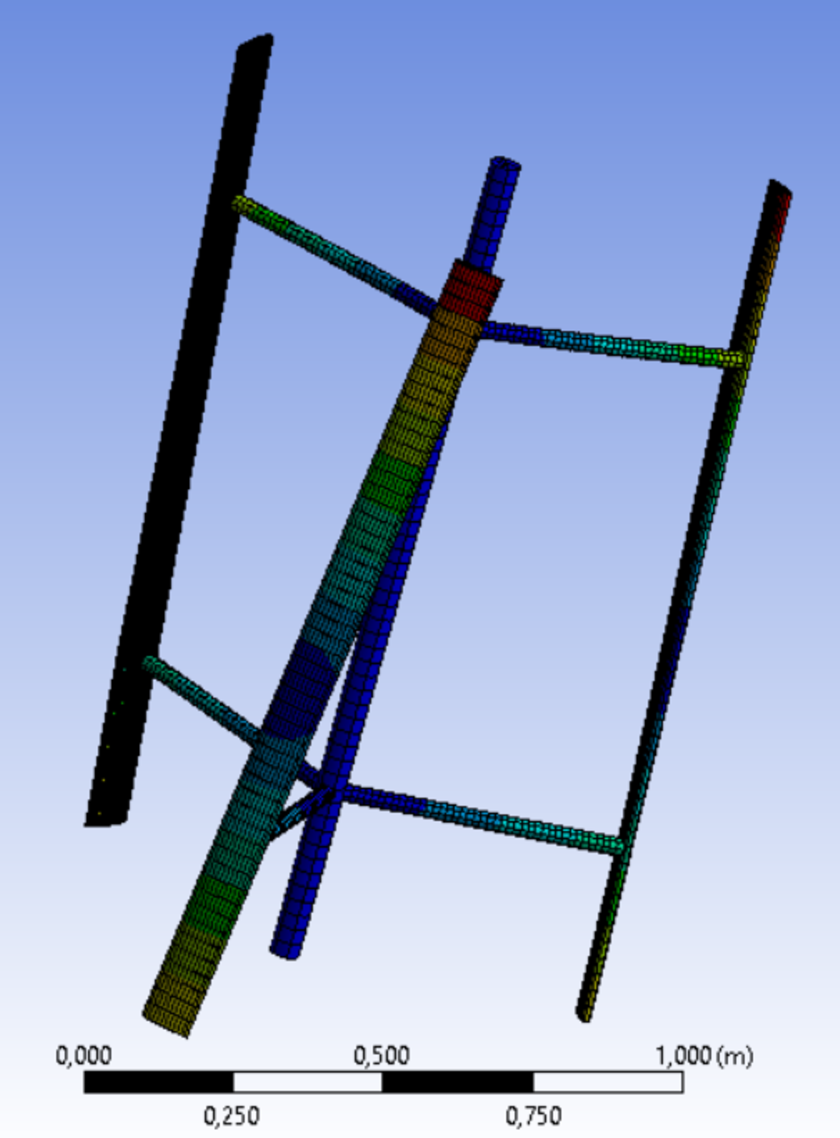
\includegraphics[width=0.95\textwidth]{figuras/resultmodalmacico6.pdf}
		\caption{Sexto modo.}
		\label{subfig:resultmodomacicomodo6}
	\end{subfigure}		
	\fonte{Autoria própria.}
\end{figure}


\section{Double-multiple streamtube model}
\label{sec:resultdmsm}

Em termos de torque, a \autoref{fig:resultCtPaFrontPost} apresenta o gráfico da coeficiente de torque para uma pá, onde é possível verificar que uma maior quantidade de torque é extraído no primeiro meio ciclo (0 - 180 graus) quando comparado com o segundo (180 - 360 graus).

\begin{figure}
	\centering
	\caption{Coeficiente de torque para uma pá.}
	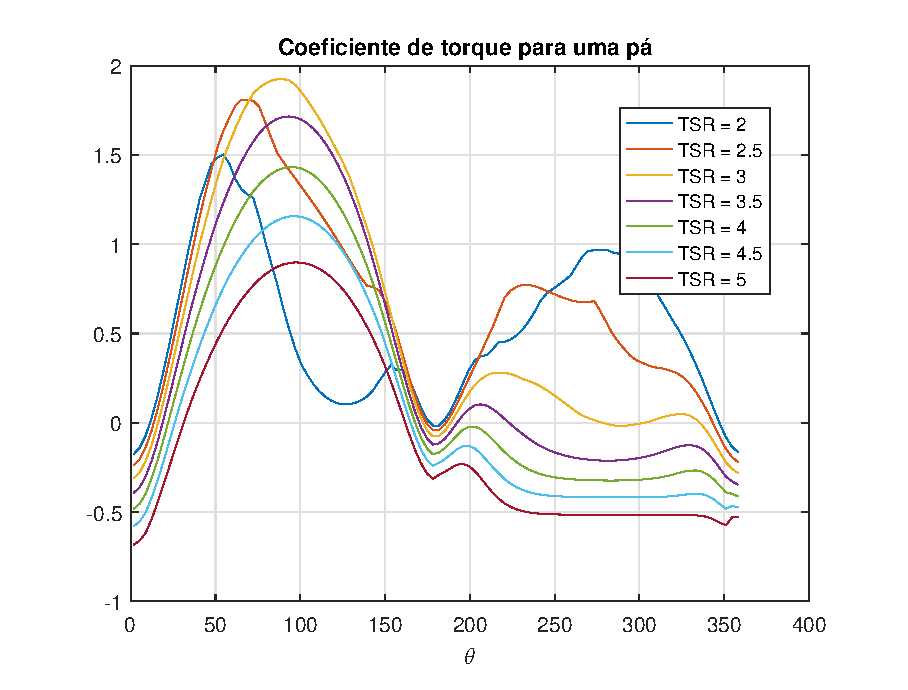
\includegraphics[width=0.8\textwidth]{figuras/resultCtPaFrontPost.eps}
	\fonte{Autoria própria.}
	\label{fig:resultCtPaFrontPost}
\end{figure}

\section{Próximas etapas}
\label{sec:trabalhosFutuross}

Os próximos passos a serem feitos estão sintetizados na \autoref{tab:cronograma}.

\begin{table}[H]
	\centering
	\caption{Cronograma.}
	\label{tab:cronograma}
	    \begin{tabular}{l c c c c c c}
        \hline TAREFA & SEM 1 & SEM 2 & SEM 3 & SEM 4 & SEM 5 & SEM 6\\
        \hline        
		Verificação da influencia da água & X & & & & & \\
		Acoplamento trem de potência & X & X & X & & & \\
		Elaboração e submissão de artigo & & & X & X & X &\\
		Redação final & X& X& X& X & X & X\\
		Submissão de versão final & & & & & & X \\
		\hline
    \end{tabular}

	\fonte{Autoria Própria.}
\end{table}

\begin{quadro}[!htb]
	\centering
	\caption{Exemplo de Quadro.\label{qua:quadro-exemplo1}}
	\begin{tabular}{|p{7cm}|p{7cm}|}
		\hline
		\textbf{BD Relacionais} & \textbf{BD Orientados a Objetos} \\
		\hline
		Os dados são passivos, ou seja, certas operações limitadas podem ser automaticamente acionadas quando os dados são usados. Os dados são ativos, ou seja, as solicitações fazem com que os objetos executem seus métodos. & Os processos que usam dados mudam constantemente. \\
		\hline
	\end{tabular}
	\fonte{XXXXXXXXXXXX.}
\end{quadro}

\end{comment}